%%%%%%%%%%%%%%%%%%%%%%%%%%%%%%%%%%%%%%%%%
% Short Sectioned Assignment
% LaTeX Template
% Version 1.0 (5/5/12)
%
% This template has been downloaded from:
% http://www.LaTeXTemplates.com
%
% Original author:
% Frits Wenneker (http://www.howtotex.com)
%
% License:
% CC BY-NC-SA 3.0 (http://creativecommons.org/licenses/by-nc-sa/3.0/)
%
%%%%%%%%%%%%%%%%%%%%%%%%%%%%%%%%%%%%%%%%%

%----------------------------------------------------------------------------------------
%	PACKAGES AND OTHER DOCUMENT CONFIGURATIONS
%----------------------------------------------------------------------------------------

\documentclass[paper=a4, fontsize=11pt]{scrartcl} % A4 paper and 11pt font size

\usepackage{fourier} % Use the Adobe Utopia font for the document - comment this line to return to the LaTeX default
\usepackage[french]{babel} % English language/hyphenation
\usepackage{amsmath,amsfonts,amsthm} % Math packages

\usepackage{lipsum} % Used for inserting dummy 'Lorem ipsum' text into the template
\usepackage{graphicx}
\usepackage{sectsty} % Allows customizing section commands
\allsectionsfont{\centering \normalfont\scshape} % Make all sections centered, the default font and small caps

\usepackage{fancyhdr} % Custom headers and footers
\pagestyle{fancyplain} % Makes all pages in the document conform to the custom headers and footers
\fancyhead{} % No page header - if you want one, create it in the same way as the footers below
\fancyfoot[L]{} % Empty left footer
\fancyfoot[C]{} % Empty center footer
\fancyfoot[R]{\thepage} % Page numbering for right footer
\renewcommand{\headrulewidth}{0pt} % Remove header underlines
\renewcommand{\footrulewidth}{0pt} % Remove footer underlines
\setlength{\headheight}{13.6pt} % Customize the height of the header

\numberwithin{equation}{section} % Number equations within sections (i.e. 1.1, 1.2, 2.1, 2.2 instead of 1, 2, 3, 4)
\numberwithin{figure}{section} % Number figures within sections (i.e. 1.1, 1.2, 2.1, 2.2 instead of 1, 2, 3, 4)
\numberwithin{table}{section} % Number tables within sections (i.e. 1.1, 1.2, 2.1, 2.2 instead of 1, 2, 3, 4)

\setlength\parindent{0pt} % Removes all indentation from paragraphs - comment this line for an assignment with lots of text

%----------------------------------------------------------------------------------------
%	TITLE SECTION
%----------------------------------------------------------------------------------------

\newcommand{\horrule}[1]{\rule{\linewidth}{#1}} % Create horizontal rule command with 1 argument of height

\title{	
\normalfont \normalsize 
\textsc{Ecole Centrale de Nantes} \\ [25pt] % Your university, school and/or department name(s)
\horrule{0.5pt} \\[0.4cm] % Thin top horizontal rule
\huge Option Informatique - Corrigé TD MADIS \\ % The assignment title
\horrule{2pt} \\[0.5cm] % Thick bottom horizontal rule
}

%\author{Durée 1h - Aucun document autorisé} % Your name

%\date{\normalsize\today} % Today's date or a custom date

\begin{document}

\maketitle % Print the title

\section{Grossiste en fleurs}

La modélisation du problème sous forme de graphe est très simple, la seule astuce consiste à créer un noeud artificiel T qui permettra d'additionner tout ce qui passe par le train.

Le graphe initial est représenté figure~\ref{fig:fleurs:un}.

\begin{figure}[ht]
\begin{center}
	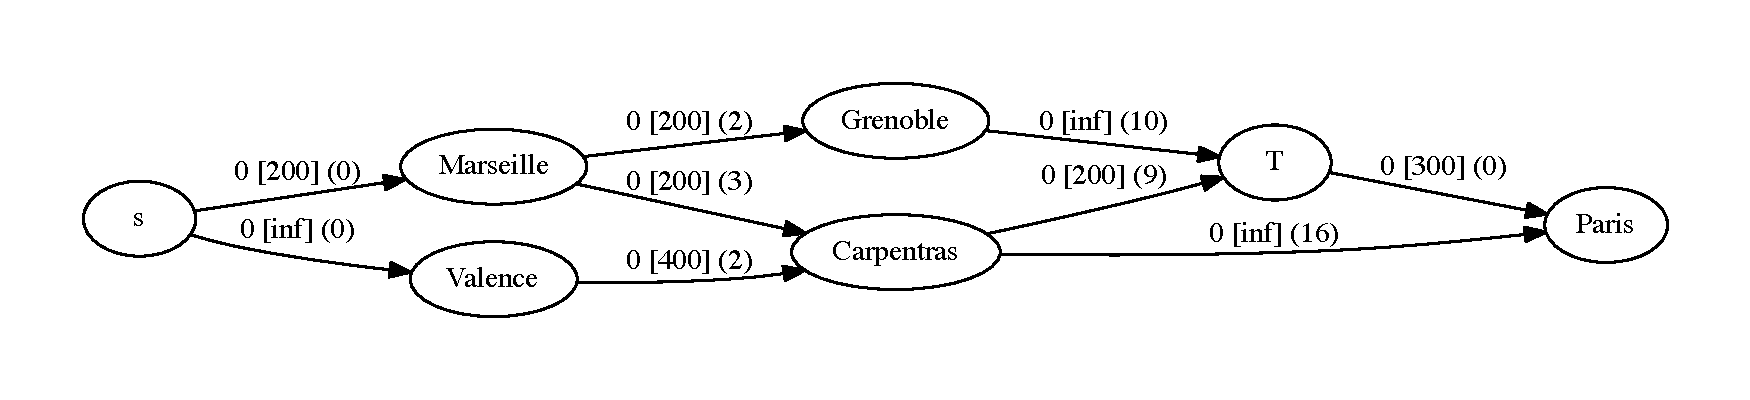
\includegraphics[width=\textwidth]{fleurs-1.pdf}
	\caption{Graphe initial}
	\label{fig:fleurs:un}
\end{center}
\end{figure}

On peut le simplifier en supprimant les sommets ayant exactement un précédesseur et un successeur, ce qui nous donne le graphe de la figure~\ref{fig:fleurs:deux} en supprimant les sommets Valence et Grenoble.


\begin{figure}[ht]
\begin{center}
	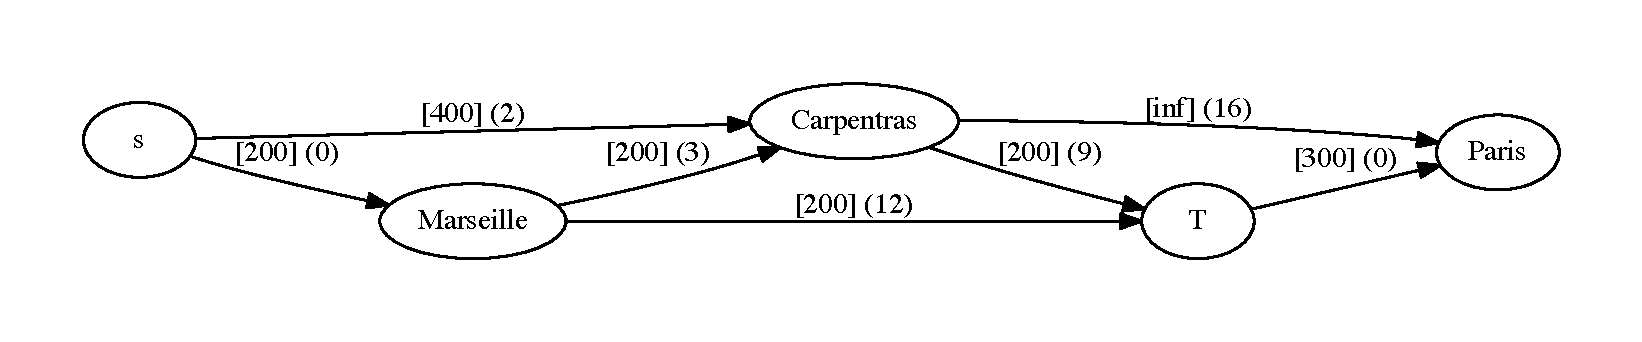
\includegraphics[width=\textwidth]{fleurs-2.pdf}
	\caption{Graphe simplifié}
	\label{fig:fleurs:deux}
\end{center}
\end{figure}

Ce graphe simplifié constitue notre premier graphe d'écart. Le plus court chemin dans celui-ci est alors s-Carpentras-T-Paris pour un coût de 11. On peut augmenter le flot de 200, ce qui nous donne le second graphe d'écart représenté figure~\ref{fig:fleurs:trois}.

\begin{figure}[ht]
\begin{center}
	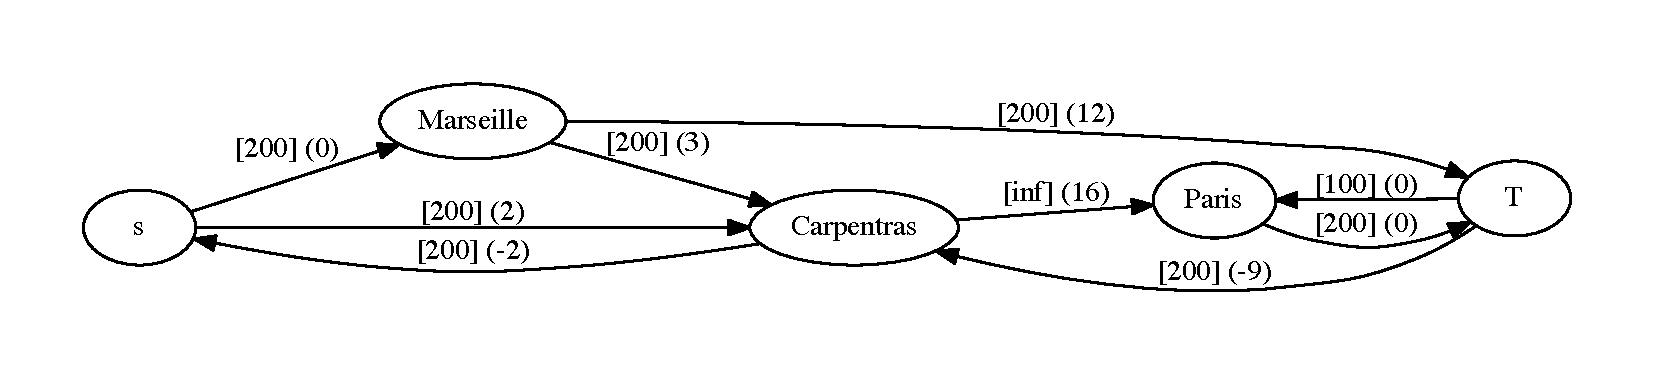
\includegraphics[width=\textwidth]{fleurs-3.pdf}
	\caption{Second graphe d'écart}
	\label{fig:fleurs:trois}
\end{center}
\end{figure}

On peut maintenant effectuer le chemin s-Marseille-T-Paris pour un coût de 12 et augmenter le flot de 100 à nouveau. Cela donne notre troisième graphe d'écart représenté figure~\ref{fig:fleurs:quatre}.

\begin{figure}[htbp]
\begin{center}
	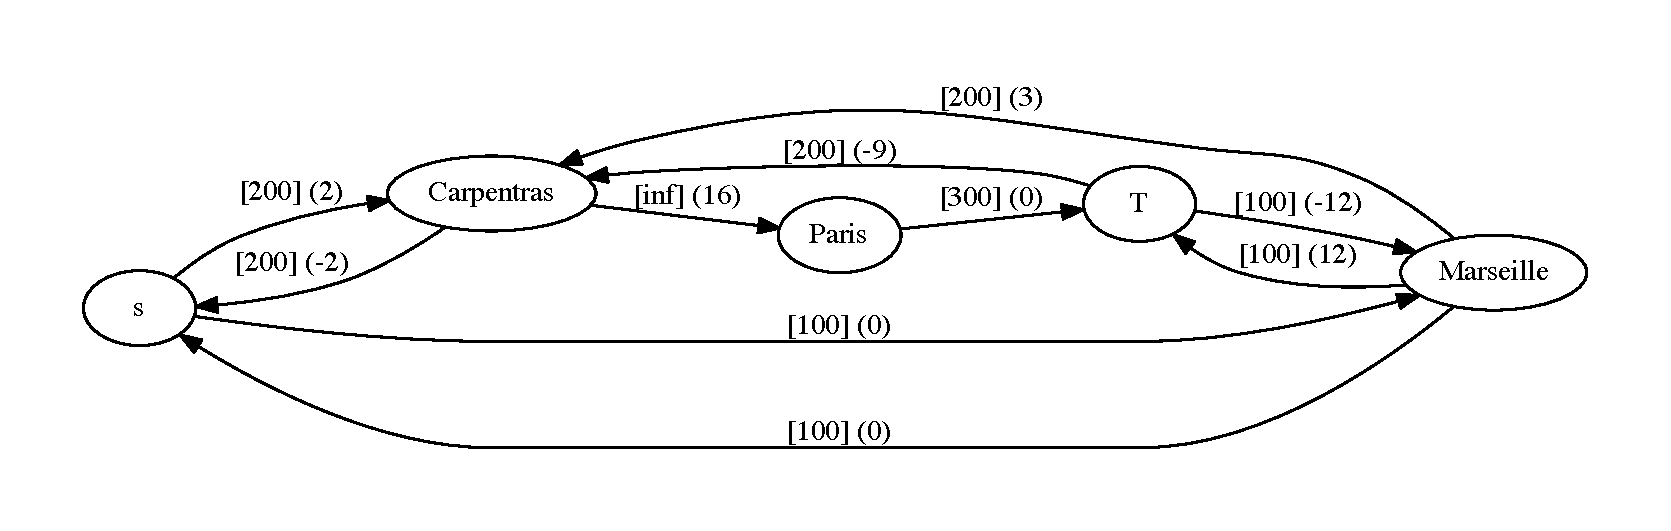
\includegraphics[width=\textwidth]{fleurs-4.pdf}
	\caption{Troisième graphe d'écart}
	\label{fig:fleurs:quatre}
\end{center}
\end{figure}

Le plus court chemin est alors s-Carpentras-Paris qui a un coût de 18 et permet d'augmenter le flot de 200. Le quatrième graphe d'écart est représenté figure~\ref{fig:fleurs:cinq}.

\begin{figure}[h]
\begin{center}
	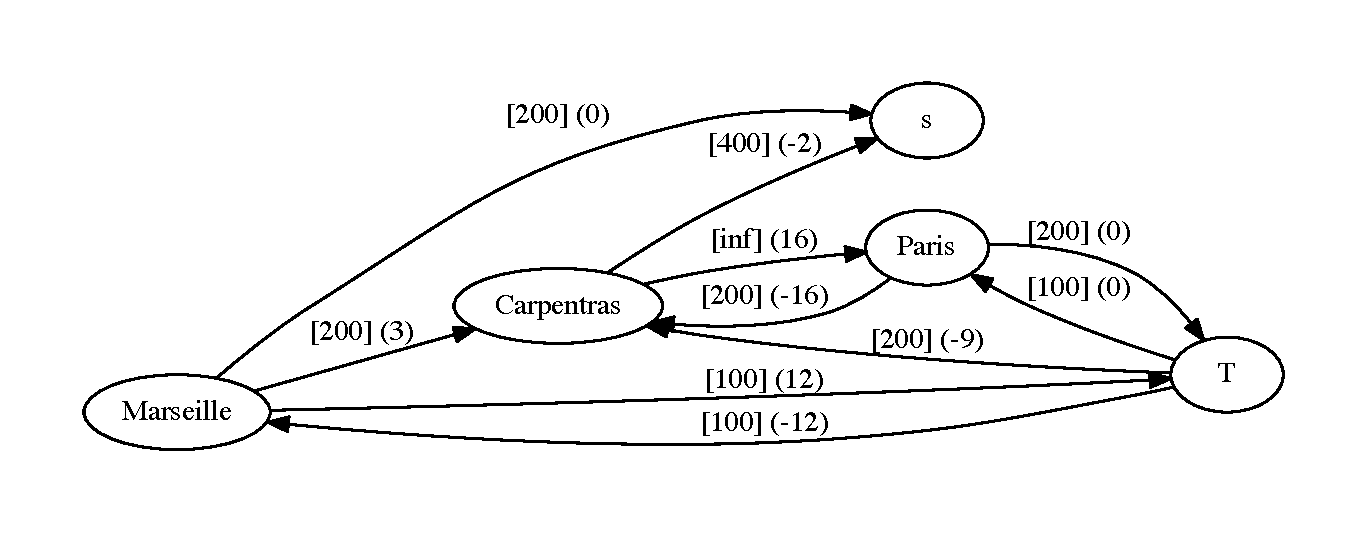
\includegraphics[width=\textwidth]{fleurs-5.pdf}
	\caption{Quatrième graphe d'écart}
	\label{fig:fleurs:cinq}
\end{center}
\end{figure}

Dernier chemin possible : s-Marseille-Carpentras-Paris pour un coût de 19 et une augmentation de flot de 100. Le cinquième graphe d'écart de la figure~\ref{fig:fleurs:six} n'a plus de chemin de s vers Paris.

\begin{figure}[h]
\begin{center}
	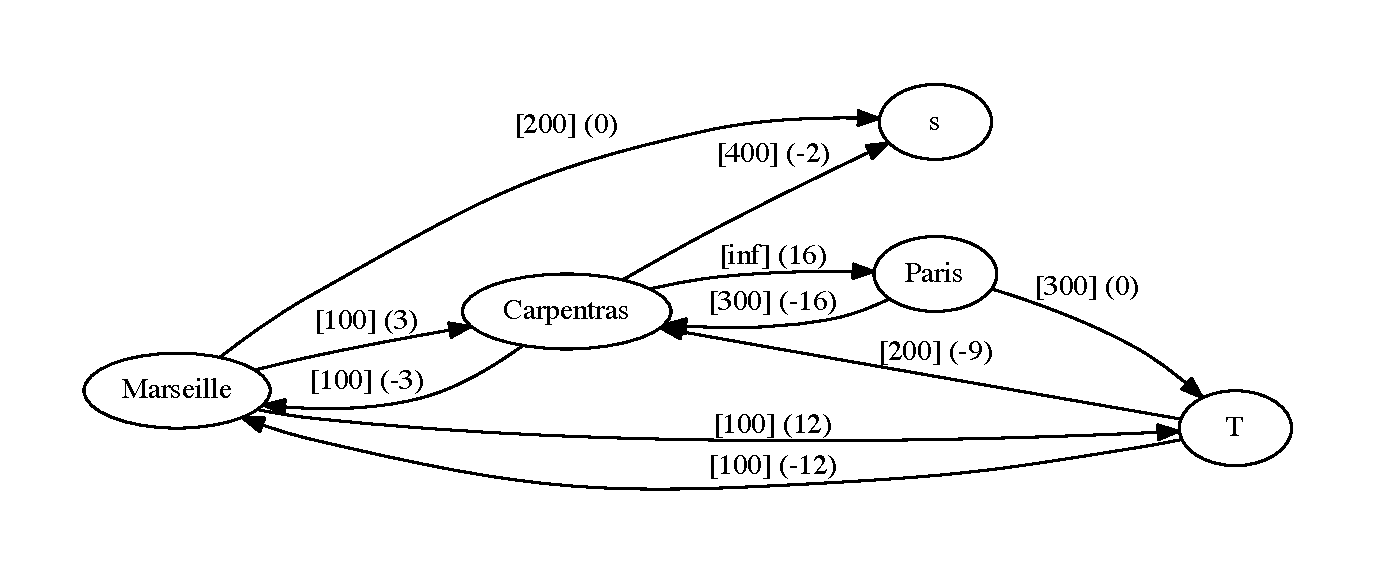
\includegraphics[width=\textwidth]{fleurs-6.pdf}
	\caption{Cinquième graphe d'écart}
	\label{fig:fleurs:six}
\end{center}
\end{figure}

Le flot total est de 600 pour un coût total de 8900.


\end{document}
%%% Local Variables: 
%%% mode: latex
%%% TeX-master: t
%%% End: 
